\section{Possible performance gains for loading models from local key-value data stores}

In this section, we analyse the performance gains from optimal model fragmentation. Even though these gains will never be achievable for real applications (in most cases), the results in this section provide a theoretical lower bound. The results also help to benchmark (existing) fragmentation strategies. 

\subsection{Optimal Fragmentation for non Distributed and Unordered Data Stores}

First, we need to define a few functions that provide the performance of all operations involved in loading a model. We define the \emph{local load} function $ll$ that determines how long it takes to load a model of a given $size$  from a local data store:

$$ll:size\rightarrow t=\mathcal{O}\left(size\right)$$

The next function \emph{find entry local} $fl$ determines how long it takes to find an entry in a local key-value data store based on the number of key $\#keys$, i.e. number of entries:

$$fl:\#keys\rightarrow t=\mathcal{O}log(\#keys)$$

We will use the following parameters: The total model $size$, the average number of objects per entry $ope$, the size of the model to load $load$, and $part$ the average percentage of an entry's objects that belong to the loaded model if at least one object is part of the loaded model.

The time $t$ to load a model with this parameters is:

\begin{eqnarray*}
t&=&\frac{load}{part*ope}\left(fl(\frac{size}{ope}) + ll(ope)\right)\\
&=&\mathcal{O}\frac{load}{part*ope}\left(log(\frac{size}{ope})+ope\right)\\
\end{eqnarray*}

The two extreme examples are: (only one big entry) $ope=size$, $part=load/size$, $t=\mathcal{O}\left(size\right)$, and (one object per entry) $ope=1$, $part=1$, $t=\mathcal{O}\left(load\left(log(size)+1\right)\right)$. 

\subsubsection{Analysis}
In the optimal model distribution (one only wants to load models that exactly constitute one entry) $ope=load$ and $part=1$ the time is $t=\mathcal{O}\left(log(\frac{size}{load})+load\right)$.

\begin{figure}
  \centering
  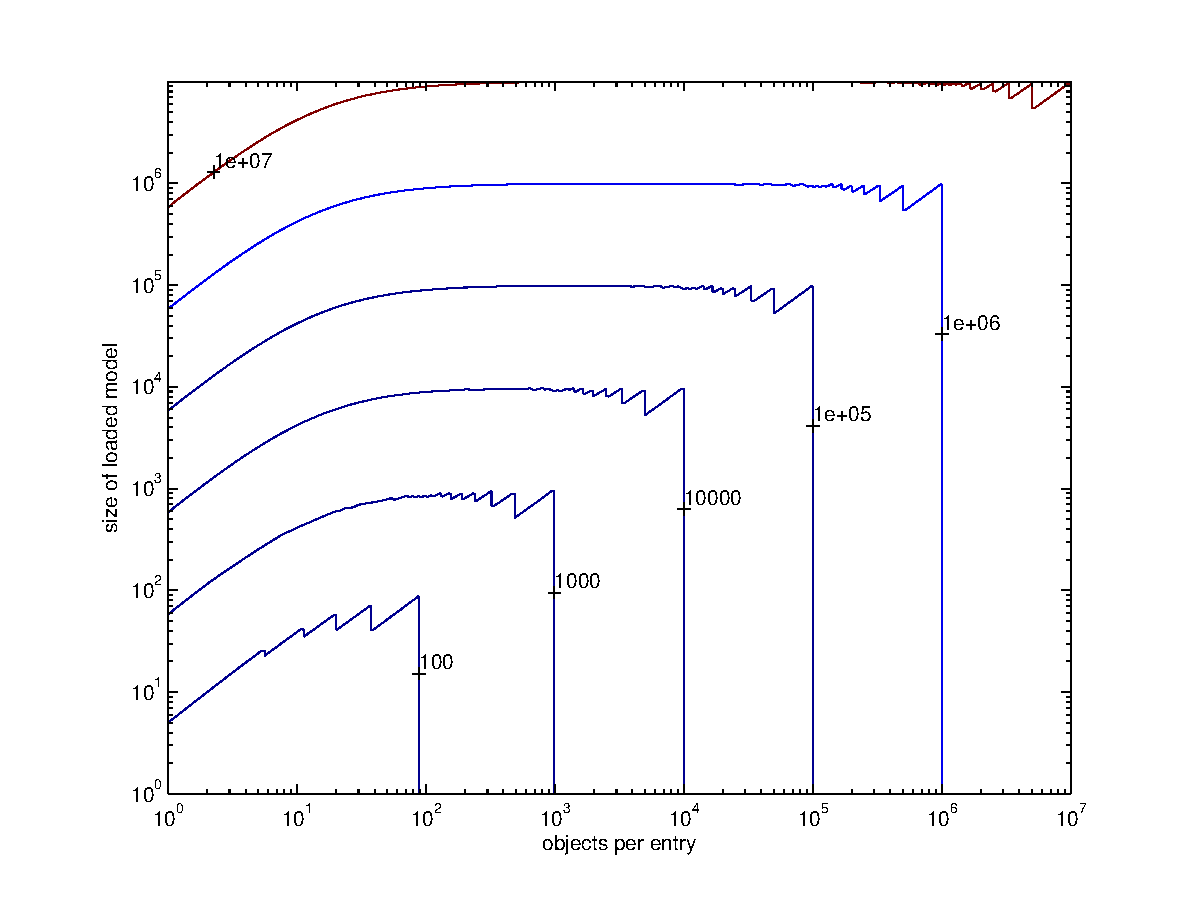
\includegraphics[width=0.65\linewidth]{figures/optimal_load_times}
  \caption{Load times}
  \label{fig:optimal_load_times}
\end{figure}

The plot in Fig.~\ref{fig:optimal_load_times} shows the relation between objects per entry, load size, and the time it takes to load. The contours show loads that take the same time. The plot does not account for any $ll=m*size+n$ and $fl=m*log(\#keys)+n$ factors ($m,n$). Depending on actual factors (see next section) the linear or logarithmic parts of the contours are more or less dominant. If parsing is relatively slow, fragmentation becomes more important (linear parts of contours are longer), if accessing the data-base becomes relatively slow, fragmentation becomes less relevant and generally large object per entry numbers are more desirable (logarithmic parts of contours are longer).

\subsubsection{Measurements}

We measured the performance of EMF parsing (depending on model size) and HBase data store access (depending on number of data store entries). The results are shown in Fig.~\ref{fig:optimal_load_times}. As expected the parsing performance is linear and the data store access behaves logarithmic. The plot in Fig.~\ref{fig:optimal_load_times_measured} is similar to Fig.~\ref{fig:optimal_load_times}, but uses $ll$ and $fl$ factors based on the measurements (actually the interpolated functions shown as lines in the plots).  

From this plot, we can see what fragmentation allows compared to no fragmentation ($ope=size$) or complete fragmentation ($ope=1$). No fragmentation always takes the full time (10s in this scenario). Of course optimal results can be obtained if ($load=ope$). This optimal result allows to load models a 1000 times bigger at the same time than total fragmentation. 

\begin{figure}[ht]
\begin{minipage}[b]{0.5\linewidth}
\centering
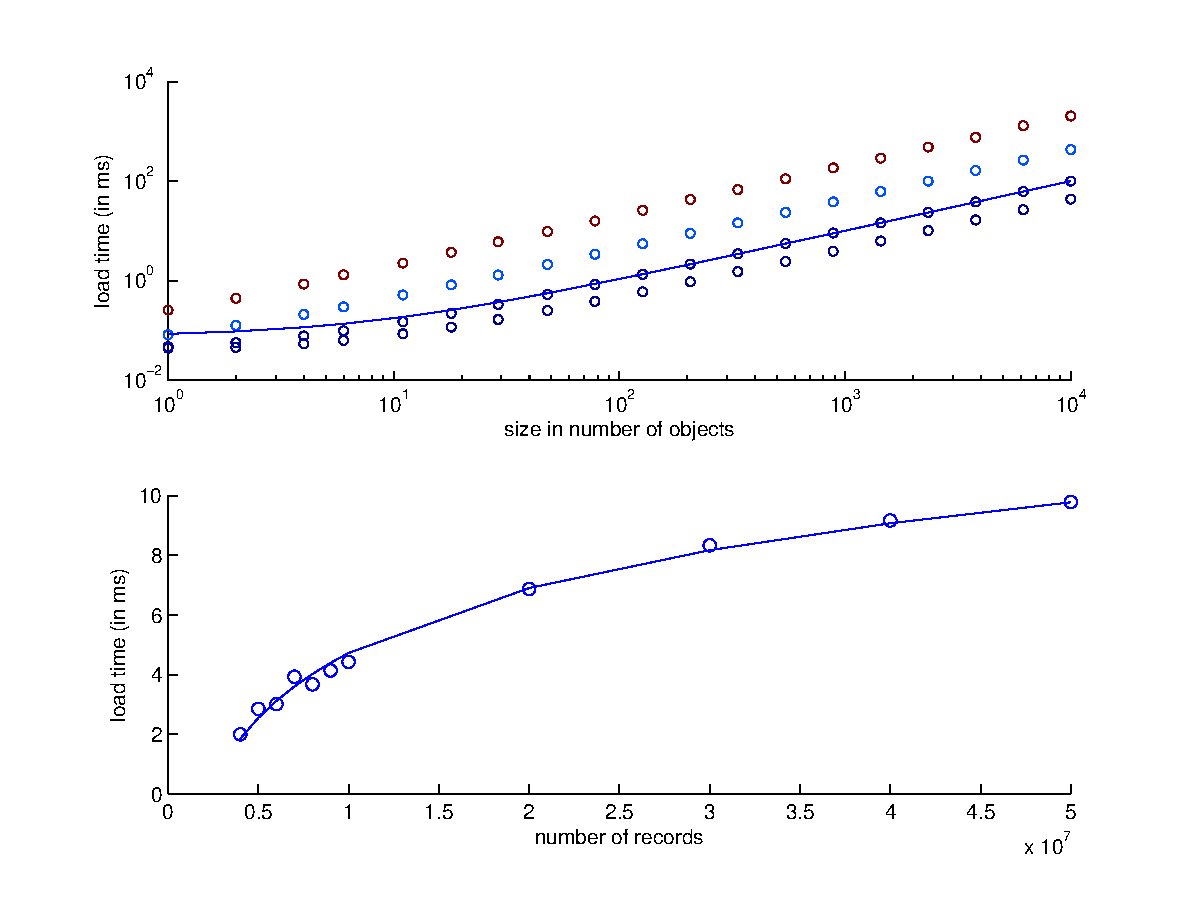
\includegraphics[width=\linewidth]{figures/emf_hbase_performance_measured}
\caption{Measure for liner parsing performance of EMF and logarithmic access performance of HBase.}
\label{fig:figures/emf_hbase_performance_measured}
\end{minipage}
\hspace{0.5cm}
\begin{minipage}[b]{0.5\linewidth}
\centering
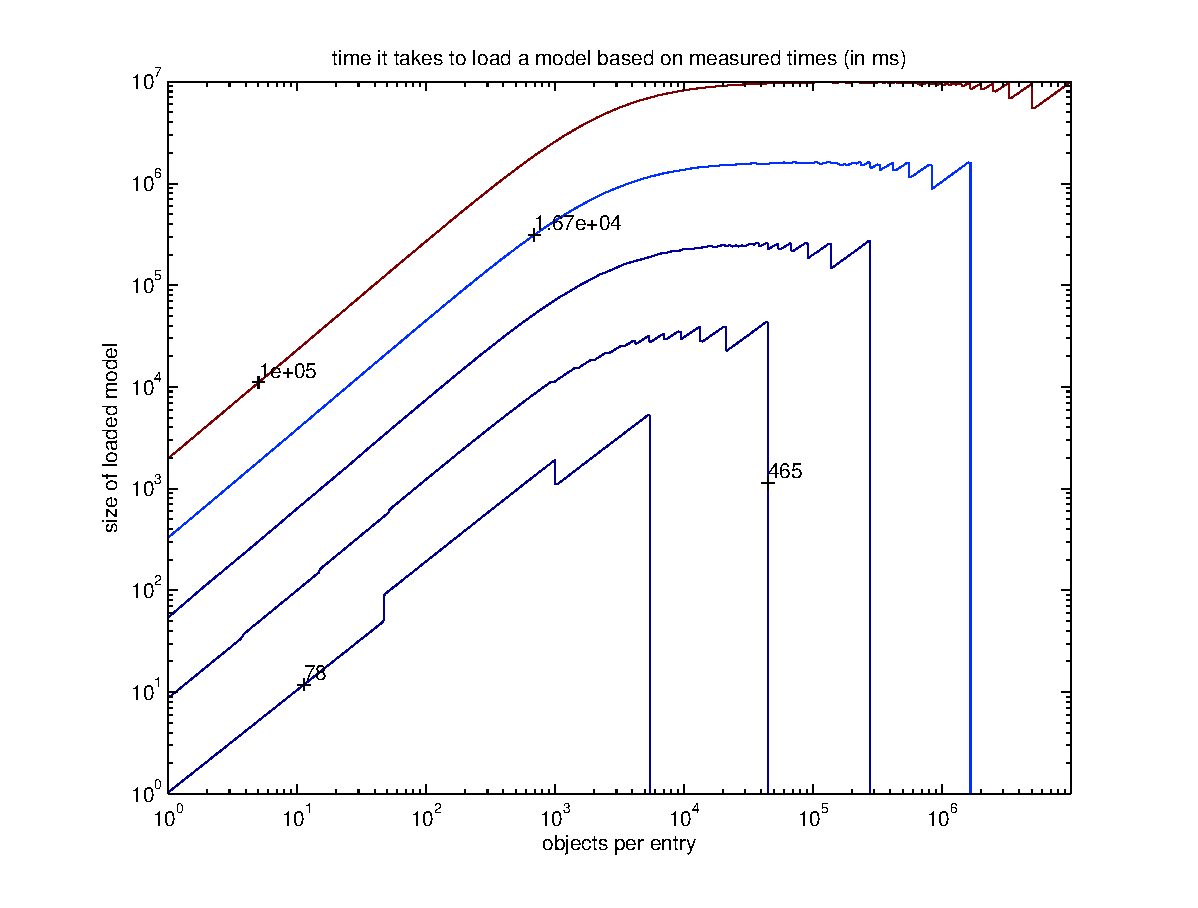
\includegraphics[width=\linewidth]{figures/optimal_load_times_measured}
\caption{Load times based on actual EMF parsing and HBase access measurements.}
\label{fig:optimal_load_times_measured}
\end{minipage}
\end{figure}

\subsection{Optimal Fragmentation in Ordered but Non Distributed Stores}

In ordered stores, entries can be scanned. If keys are chosen intelligently, a loaded model consisting of multiple fragments can still be with only one logarithmic access and subsequent scans. Assuming that all keys are always chosen in the optimal way and that the time between scans is close to 0: as long as $ope<load$ the required load time equals $ll(load)$. We can have more fine grain fragmentation without loosing performance if larger models are loaded. 

\subsection{Optimal Fragmentation in Unordered but Distributed Stores}